\chapter{Optimierung des ARM-Codes}
\label{ch:optarm}
\rm

In diesem Kapitel sollen die Anfangsbedingungen, die Ansatzpunkte, die Konzepte der durchgef�hrten Optimierungen am ARM-Code des \textit{Music Classificators} vorgestellt werden.\\
Hierzu sollen in \textbf{Kapitel \ref{sec:fset}} zuerst die Featuresets vorgestellt werden, welche f�r die Messungen der Laufzeit des Programms verwendet wurden, aus denen in \textbf{Kapitel \ref{sec:ansatz}} die wesentlichen
Bottlenecks und Optimierungspotenziale auf dem DaVinci\texttrademark extrahiert werden sollen. \textbf{Kapitel \ref{sec:optFFT}} befasst sich daraufhin den Konzepten und der Durchf�hrung von Optimierungen der FFT.

\section{Ansatzpunkte und Bottlenecks}\label{sec:ansatz}

Auf Basis der in \textbf{Kapitel \ref{sec:fset}} vorgestellten Featuresets sollen nun die vor Beginn der Optimierung durchgef�hrten Laufzeitmessungen vorgestellt und er�rtert werden. Es wurden zwei unterschiedliche Messreihen durchgef�hrt, die sich in den gew�hlten Optimierungen unterscheiden, die vom Compiler zur Compilezeit automatisch durchgef�hrt werden k�nnen. F�r die erste Messreihe wurde lediglich der Compilerflag \textit{-O3} verwendet, welches f�r die h�chste automatische Compileroptimierung steht, diese Messreihe soll f�r weitere Betrachtungen als \textit{Unoptimized} bezeichnet werden. \\
Die zweite Messreihe schlie�t die in \textbf{Kapitel \ref{subsec:neon}} vorgestellte NEON-Einheit ein. Auch f�r diese Messreihe wurden keine NEON-spezifischen Optimierungen des Codes vorgenommen, sondern nur die vom Compiler angebotene Option aktiviert, den Code w�hrend des Compilings selber f�r den NEON zu optimieren, im Weiteren wird diese Messreihe als \textit{NEON Autocompiler} bezeichnet. \\
Die Laufzeitanteile der drei Programmteile \textit{Extraction}, \textit{Processing} und \textit{Classification} sind in \textbf{Abbildung \ref{fig:ResultsMCL}} dargestellt.\\
%
\begin{figure}[htbp]
	\centering
		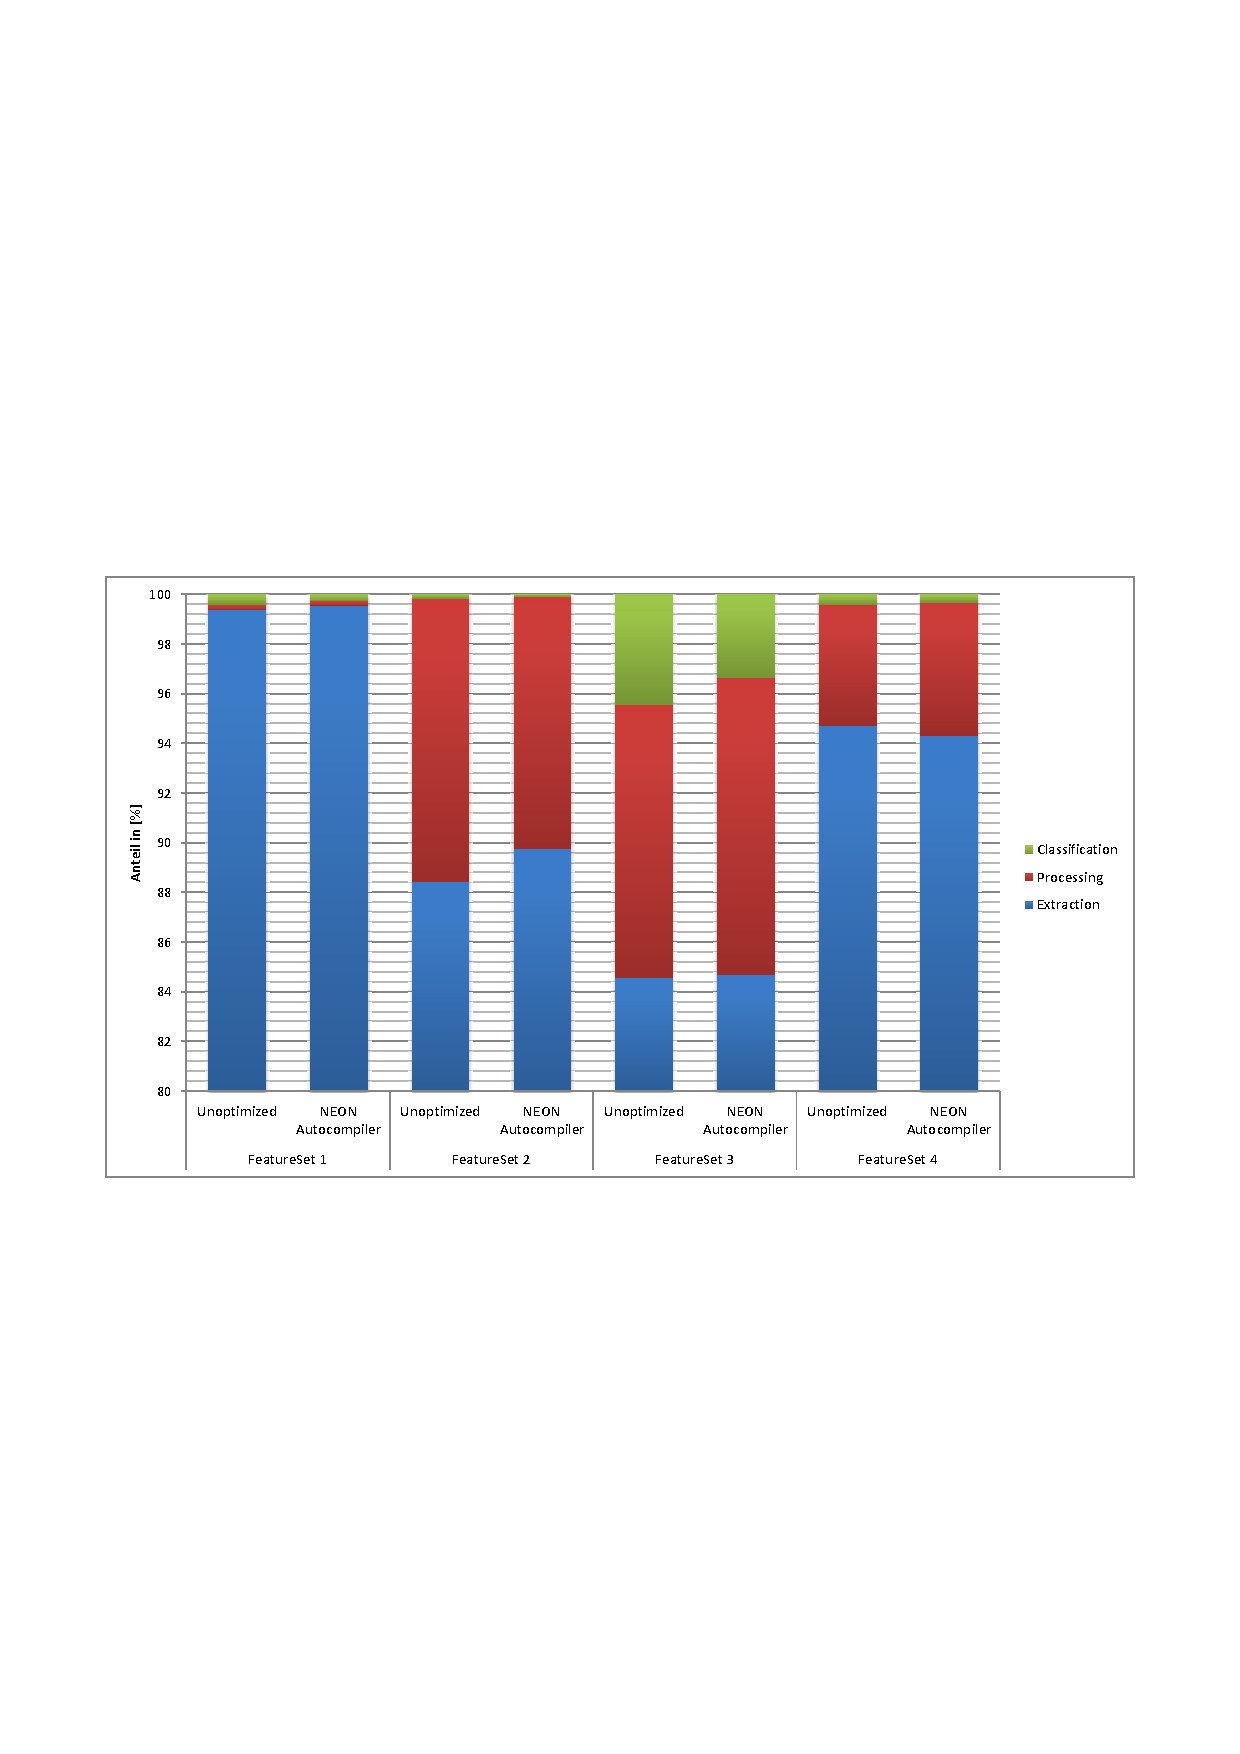
\includegraphics[width=1.00\textwidth]{../Pictures/ResultsMCL.pdf}
	\caption{Laufzeitanteile ohne manuelle Optimierung}
	\label{fig:ResultsMCL}
\end{figure}
%
Wie man leicht erkennen kann hat die Extraktion bei allen vier Featuresets mit teilweise weit �ber 80\% den gr��ten Anteil an der Laufzeit des Programms, daher wird im Nachfolgenden die Extraktion noch etwas detaillierter betrachtet werden. \\
\textbf{Abbildung \ref{fig:ResultsExtraction}} zeigt die Anteile der einzelnen Features an der Gesamtlaufzeit der Extraktion. Hier soll daran erinnert werden, dass \textit{FSet1}, \textit{FSet2} und \textit{FSet4} aus Features bestehen, die aus dem Frequenzbereich stammen, wodurch vor der Extraktion erst eine Fourier-Transformation vom Zeitbereich in diesen stattfinden muss, weshalb als weiteres "`Feature"' die FFT in der Abbildung auftaucht. Des weiteren arbeitet das Feature \textit{Ampitude of Maximum In Chromagram} aus \textit{FSet4} auf dem in \textbf{Kapitel \ref{subsubsec:cv}} vorgestellten \textit{Chroma Vector}, was dazuf�hrt, dass auch dieser in der Abbildung auftaucht.\\
%
\begin{figure}[htbp]
	\centering
		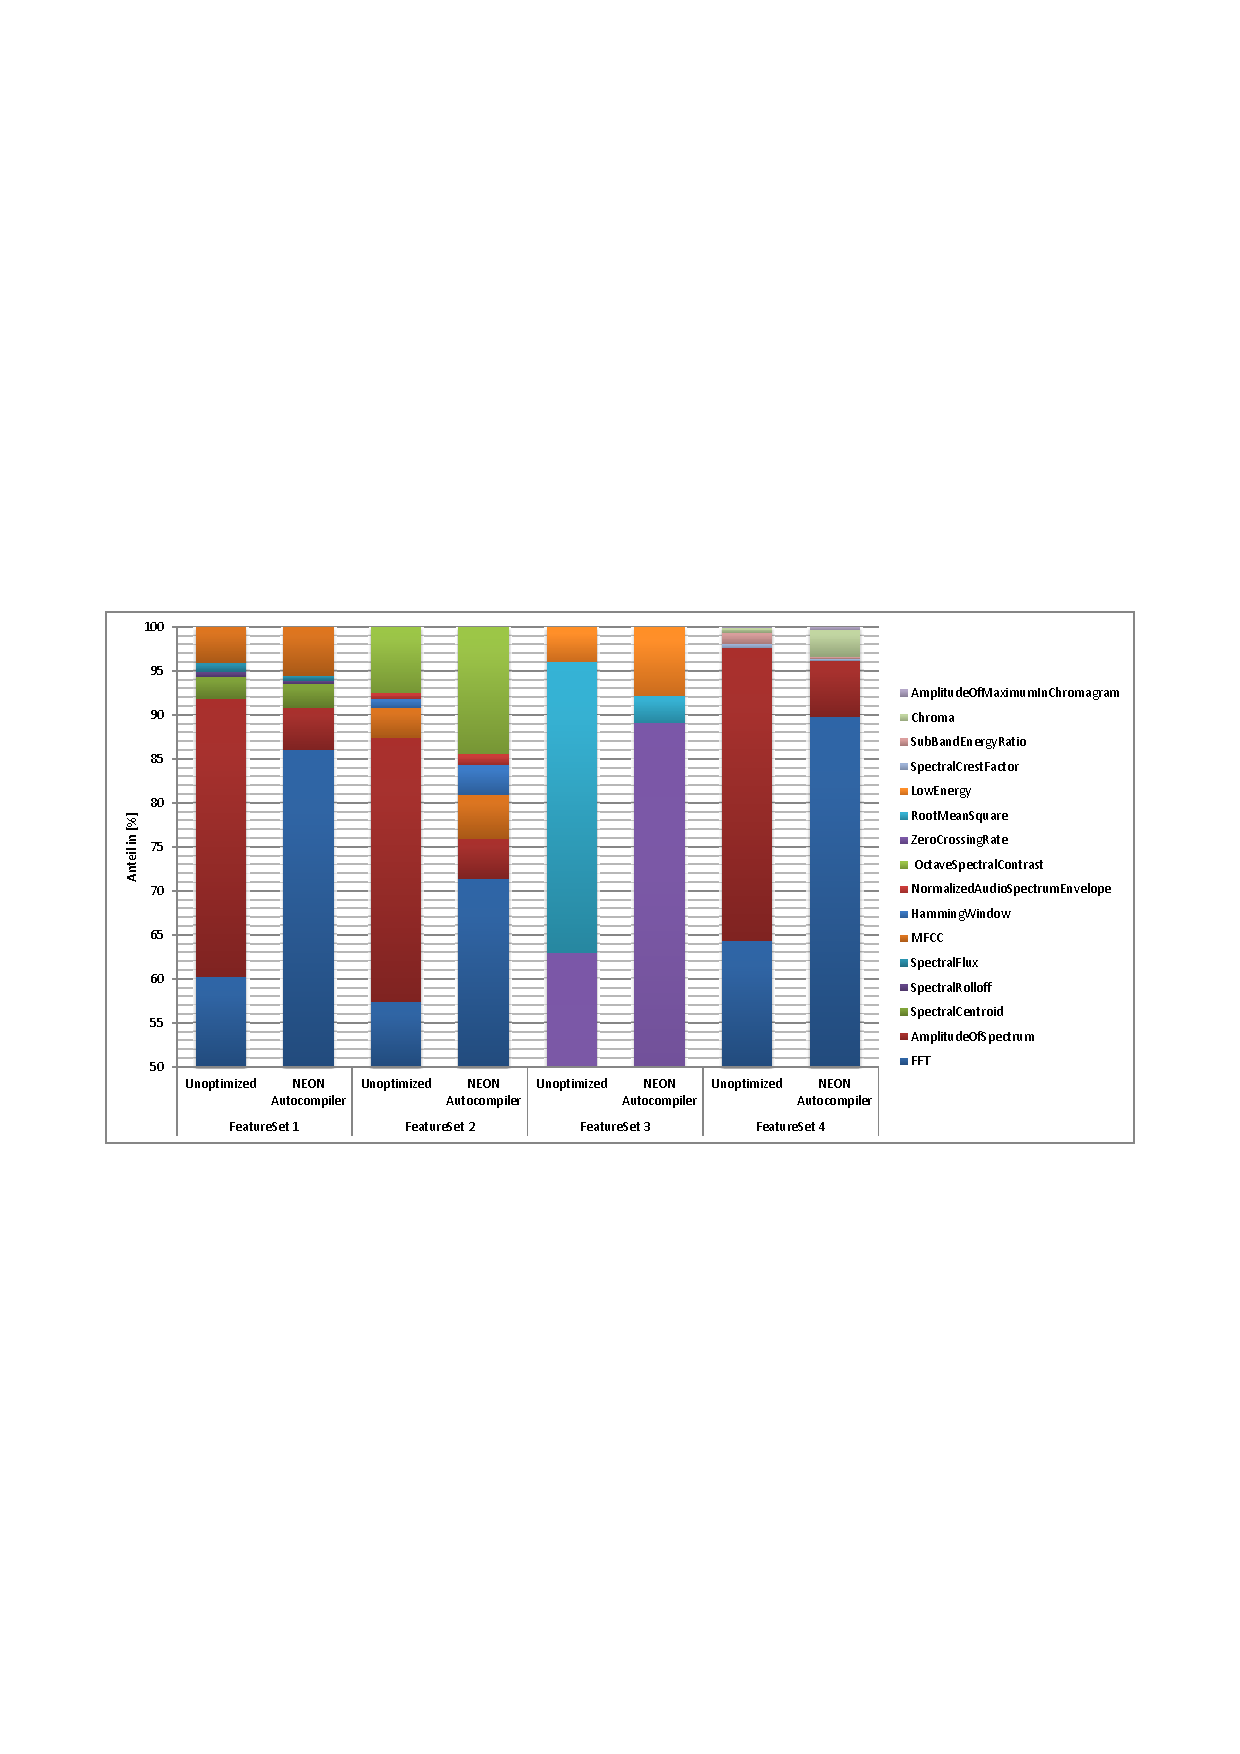
\includegraphics[width=1.00\textwidth]{../Pictures/ResultsExtraktion.pdf}
	\caption{Detaillierte Laufzeitenanteile der Extraktion ohne manuelle Optimierung}
	\label{fig:ResultsExtraction}
\end{figure}
%
Wie man der \textbf{Abbildung \ref{fig:ResultsExtraction}} entnehmen kann, hat gerade diese Transformation vom Zeit- in den Frequenzbereich den gr��ten Laufzeitbedarf, ihr Anteil liegt immer �ber 50\%. Um Irritationen zu vermeiden, soll darauf hingewiesen werden, dass sich die Laufzeit der FFT in \textit{NEON Autocompiler} nicht, wie es in der Abbildung den Anschein hat, drastisch verschlechtert hat, sondern die Verbesserungen der tats�chlichen Feature-Extraktionen sich dahingehend verbessert haben, dass die \textit{FFT} dadurch einen prozentual gr��eren Anteil einnimmt. Um genauer zu sein, hat sich in den Experimenten gezeigt, dass sich die Laufzeit der \textit{FFT} in nahezu allen F�llen fast halbiert hat.\\
Da sich gezeigt hat, dass die \textit{FFT} den gr��ten Anteil an der Laufzeit hat und das diese durch die NEON-Einheit vom Compiler schon gut optimiert werden konnte, soll im n�chsten Kapitel betrachtet werden, ob dieses durch gezielte Optimierungen bez�glich der NEON-Einheit im Code noch weiter verbessert werden kann.


\section{Optimierung der FFT}\label{sec:optFFT}
Wie im vorherigen Abschnitt gezeigt wurde, nimmt die Berechnung der \textit{FFT} die gr��ten Anteil an der Laufzeit ein. Au�erdem wurde gezeigt, dass diese ein gutes Optimierungspotenzial hinsichtlich der NEON-Einheit besitzt. Da eine NEON-Optimierung des FFT-Codes viel Zeit in Anspruch nehmen k�nnte und bereits FFT-Bibliotheken verf�gbar sind, die hinsichtlich der NEON-Einheit optimiert wurden, soll im folgenden eine dieser Bibliotheken beschrieben werden.\\
Zu den Bibliotheken die NEON-optimierten FFT-Code bereitstellen, geh�ren unter anderem \textit{"`Fastest Fourier Transformation in the West"'}, \textit{"`Fastest Fourier Transformation in the South"'} , \textit{"`Cricket FFT"'} und \textit{"`Libav"'} (\textbf{\ref{subsec:libav}}). Da jede einzelne von sich selbst behauptet den schnellsten FFT-Code zu beinhalten, aber meistens keine Benchmarks vorhanden sind, wurde f�r diese Arbeit \textit{"`Libav"'} gew�hlt, da dieses die weitverbreiteste Bibliothek ist und auch in namenhaften Programmen, wie zum Beispiel dem \textit{VideoLan Player} eingesetzt wird \cite{vlc}.

\subsection{Libav}\label{subsec:libav}

Libav beinhaltet nicht nur den in f�r diese Arbeit wichtigen FFT-Code, sondern bietet dar�ber hinaus weitere Algorithmen der Signalverarbeitung.\\
Da dar�ber hinaus in Libav mehrere FFTs zur Verf�gung gestellt werden, die f�r ganz unterschiedliche Systeme optimiert wurden, soll in diesem Kapitel nur auf den f�r ARM-Prozessoren optimierten NEON-Code eingegangen werden. 

\subsubsection{Aufbau der FFT}\label{subsubsec:libavfft}

Als erstes soll hier erw�hnt werden, das Libav zwei Ans�tze einer NEON-optimierten FFT zur Verf�gung stellt. Neben der in dieser Arbeit verwendeten floatingpoint Version ist auch noch eine fixpoint Version verf�gbar.\\
 

\subsubsection{Einbindung in den Code}\label{subsubsec:libavin}



 